\section{Результаты измерений}

Максимальное давление при пробулькивании
\[\Delta p_\text{спирт}=98\pm 1\,\text{Па}\]
Тогда диаметр иглы
\[d_0 = \frac{4\sigma}{\Delta p_\text{спирт}} = 0{,}893\pm0{,}009\,\text{мм}\]
Измерения по микроскопу дали результаты
\begin{table}[ht!]
    \centering
    \begin{tabular}{|l|l|l|l|l|}
    \hline
    $1{,}05\,\text{мм}$ & $1{,}00\,\text{мм}$ & $1{,}00\,\text{мм}$ & $0{,}95\,\text{мм}$ & $0{,}95\,\text{мм}$ \\ \hline
    \end{tabular}
\end{table}
\[d = 0{,}99\pm0{,}03\,\text{мм}\]

Перенесем иглу в колбу с водой.

Максимальное давление при пробулькивании с иглой на поверхности
\[p_1 = 294\pm 1\,\text{Па}\]
\[h_1 = 5{,}45\pm 0{,}025\,\text{см}\]

Максимальное давление при пробулькивании с утопленной иглой
\[p_2 = 451\pm 1\,\text{Па}\]
\[h_2 = 3{,}85\pm 0{,}025\,\text{см}\] 
\[\Delta h = h_1 - h_2 = 1{,}6\pm 0{,}05\,\text{см}\]
\[\Delta h = \frac{p_2 - p_1}{\rho g} = 1{,}6\pm 0{,}02\,\text{см}\]

Зависимость давления от температуры
\begin{table}[!ht]
    \centering
    \begin{tabular}{|l|l|}
    \hline
        $T,\,\text{К}$ & $l,\,\text{дел.}$ \\ \hline
        22 & 230 \\ \hline
        25.4 & 226 \\ \hline
        30.4 & 225 \\ \hline
        35.3 & 225 \\ \hline
        40.3 & 223.5 \\ \hline
        45.2 & 221.5 \\ \hline
        50 & 220 \\ \hline
        55 & 218 \\ \hline
        60 & 216 \\ \hline
    \end{tabular}
\end{table}

\[\sigma = \frac{p_2 d}{4} = 73\pm 2\,\text{мН}/\text{м}\]

\[\frac{d\sigma}{dt} = k = -0{,}177\pm0{,}002\,\text{мН}/\text{м}\cdot\text{К}\]

\begin{figure}[ht!]
    \centering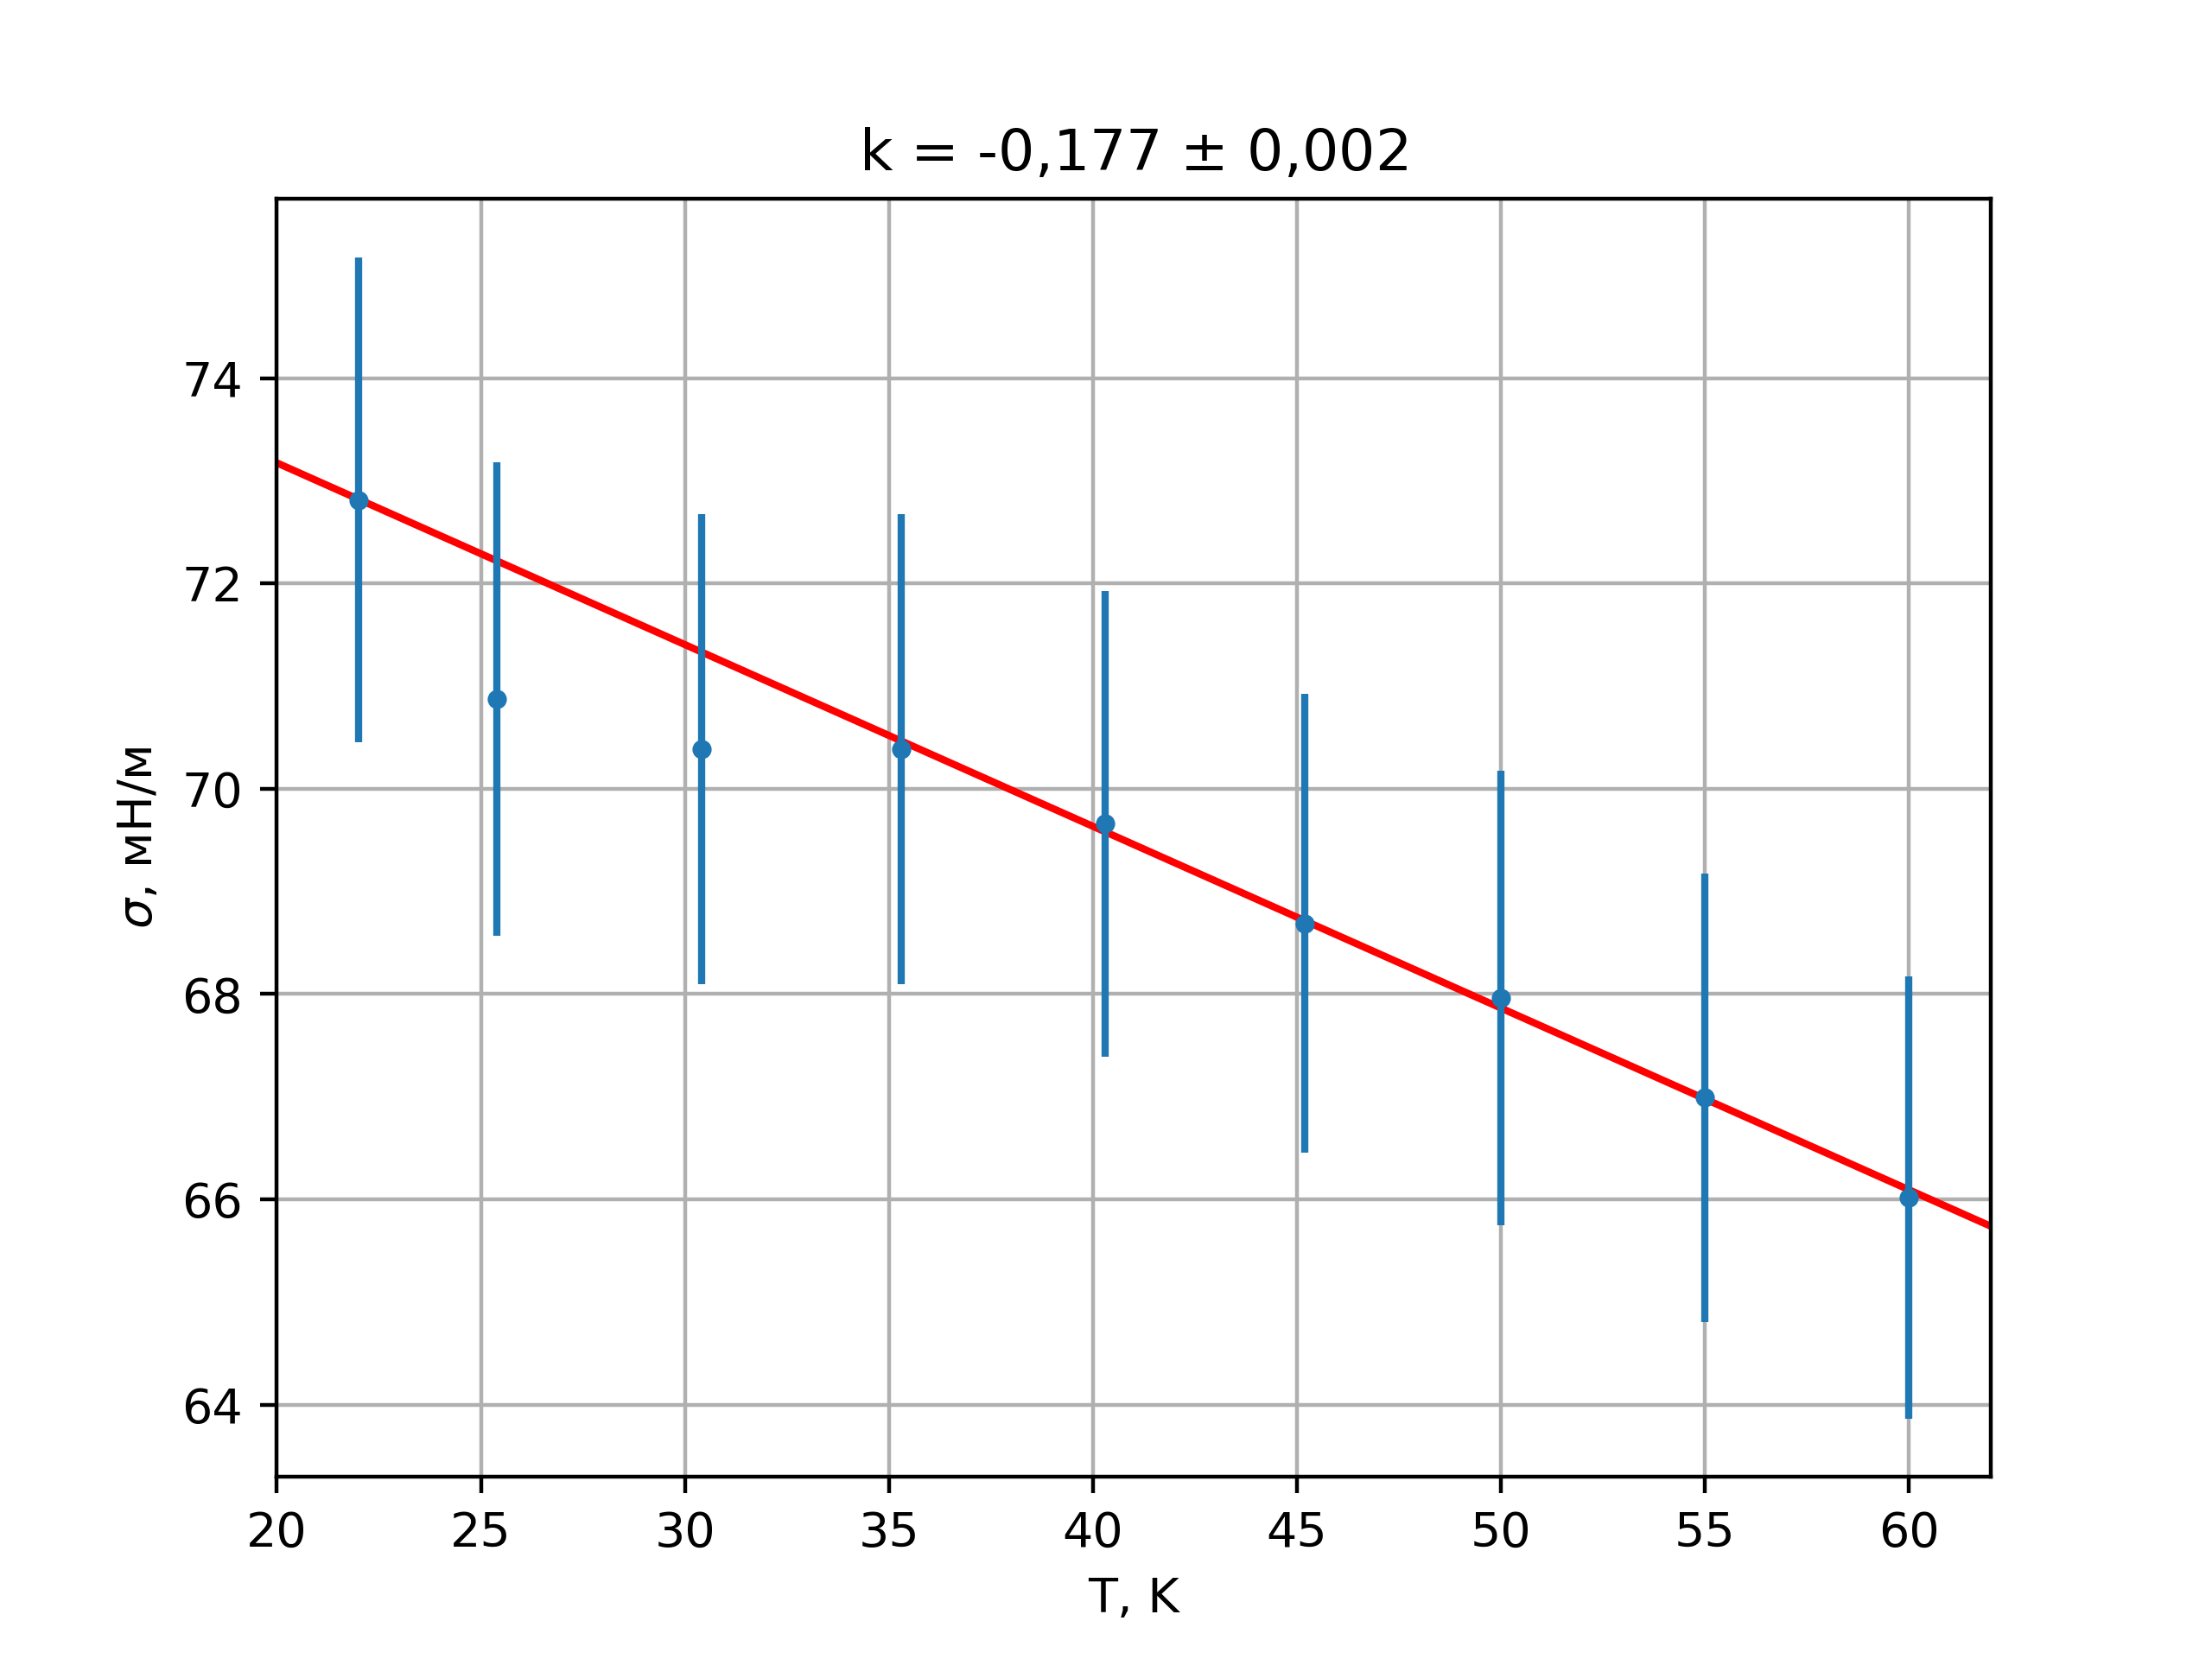
\includegraphics[width=0.8\linewidth]{img/plot1.png}
\end{figure}
\begin{figure}[ht!]
    \centering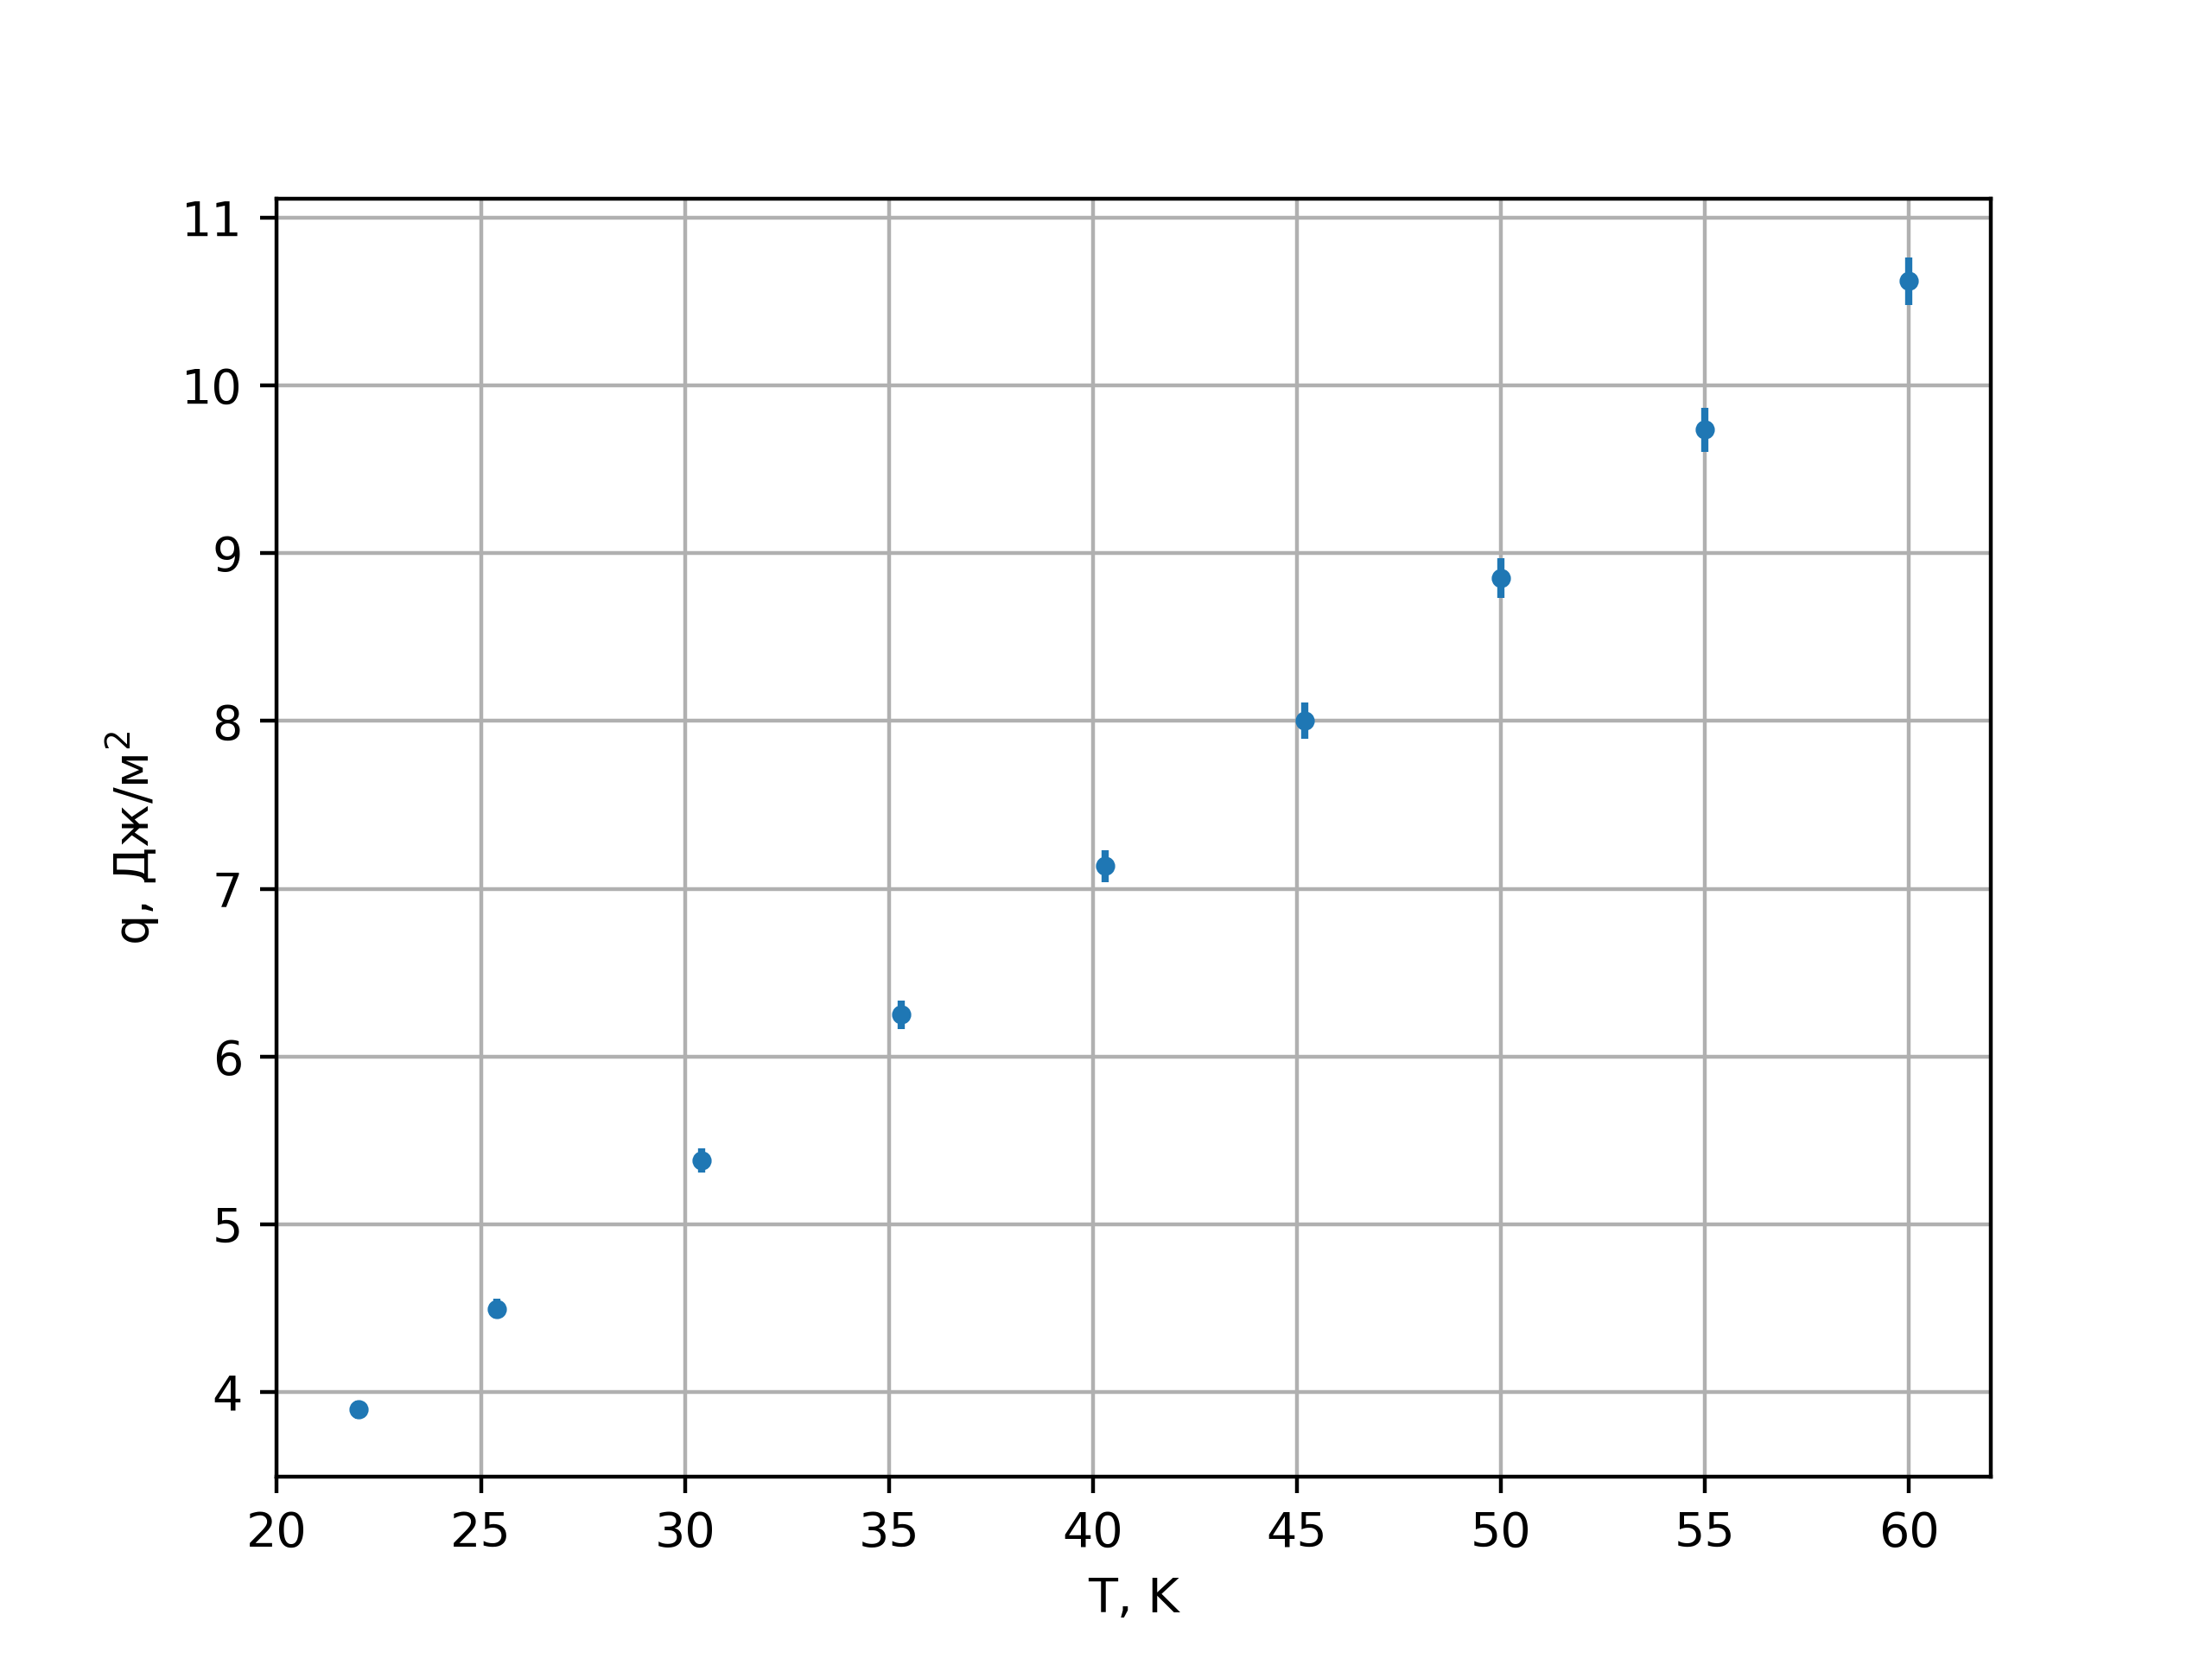
\includegraphics[width=0.8\linewidth]{img/plot2.png}
\end{figure}
\begin{figure}[ht!]
    \centering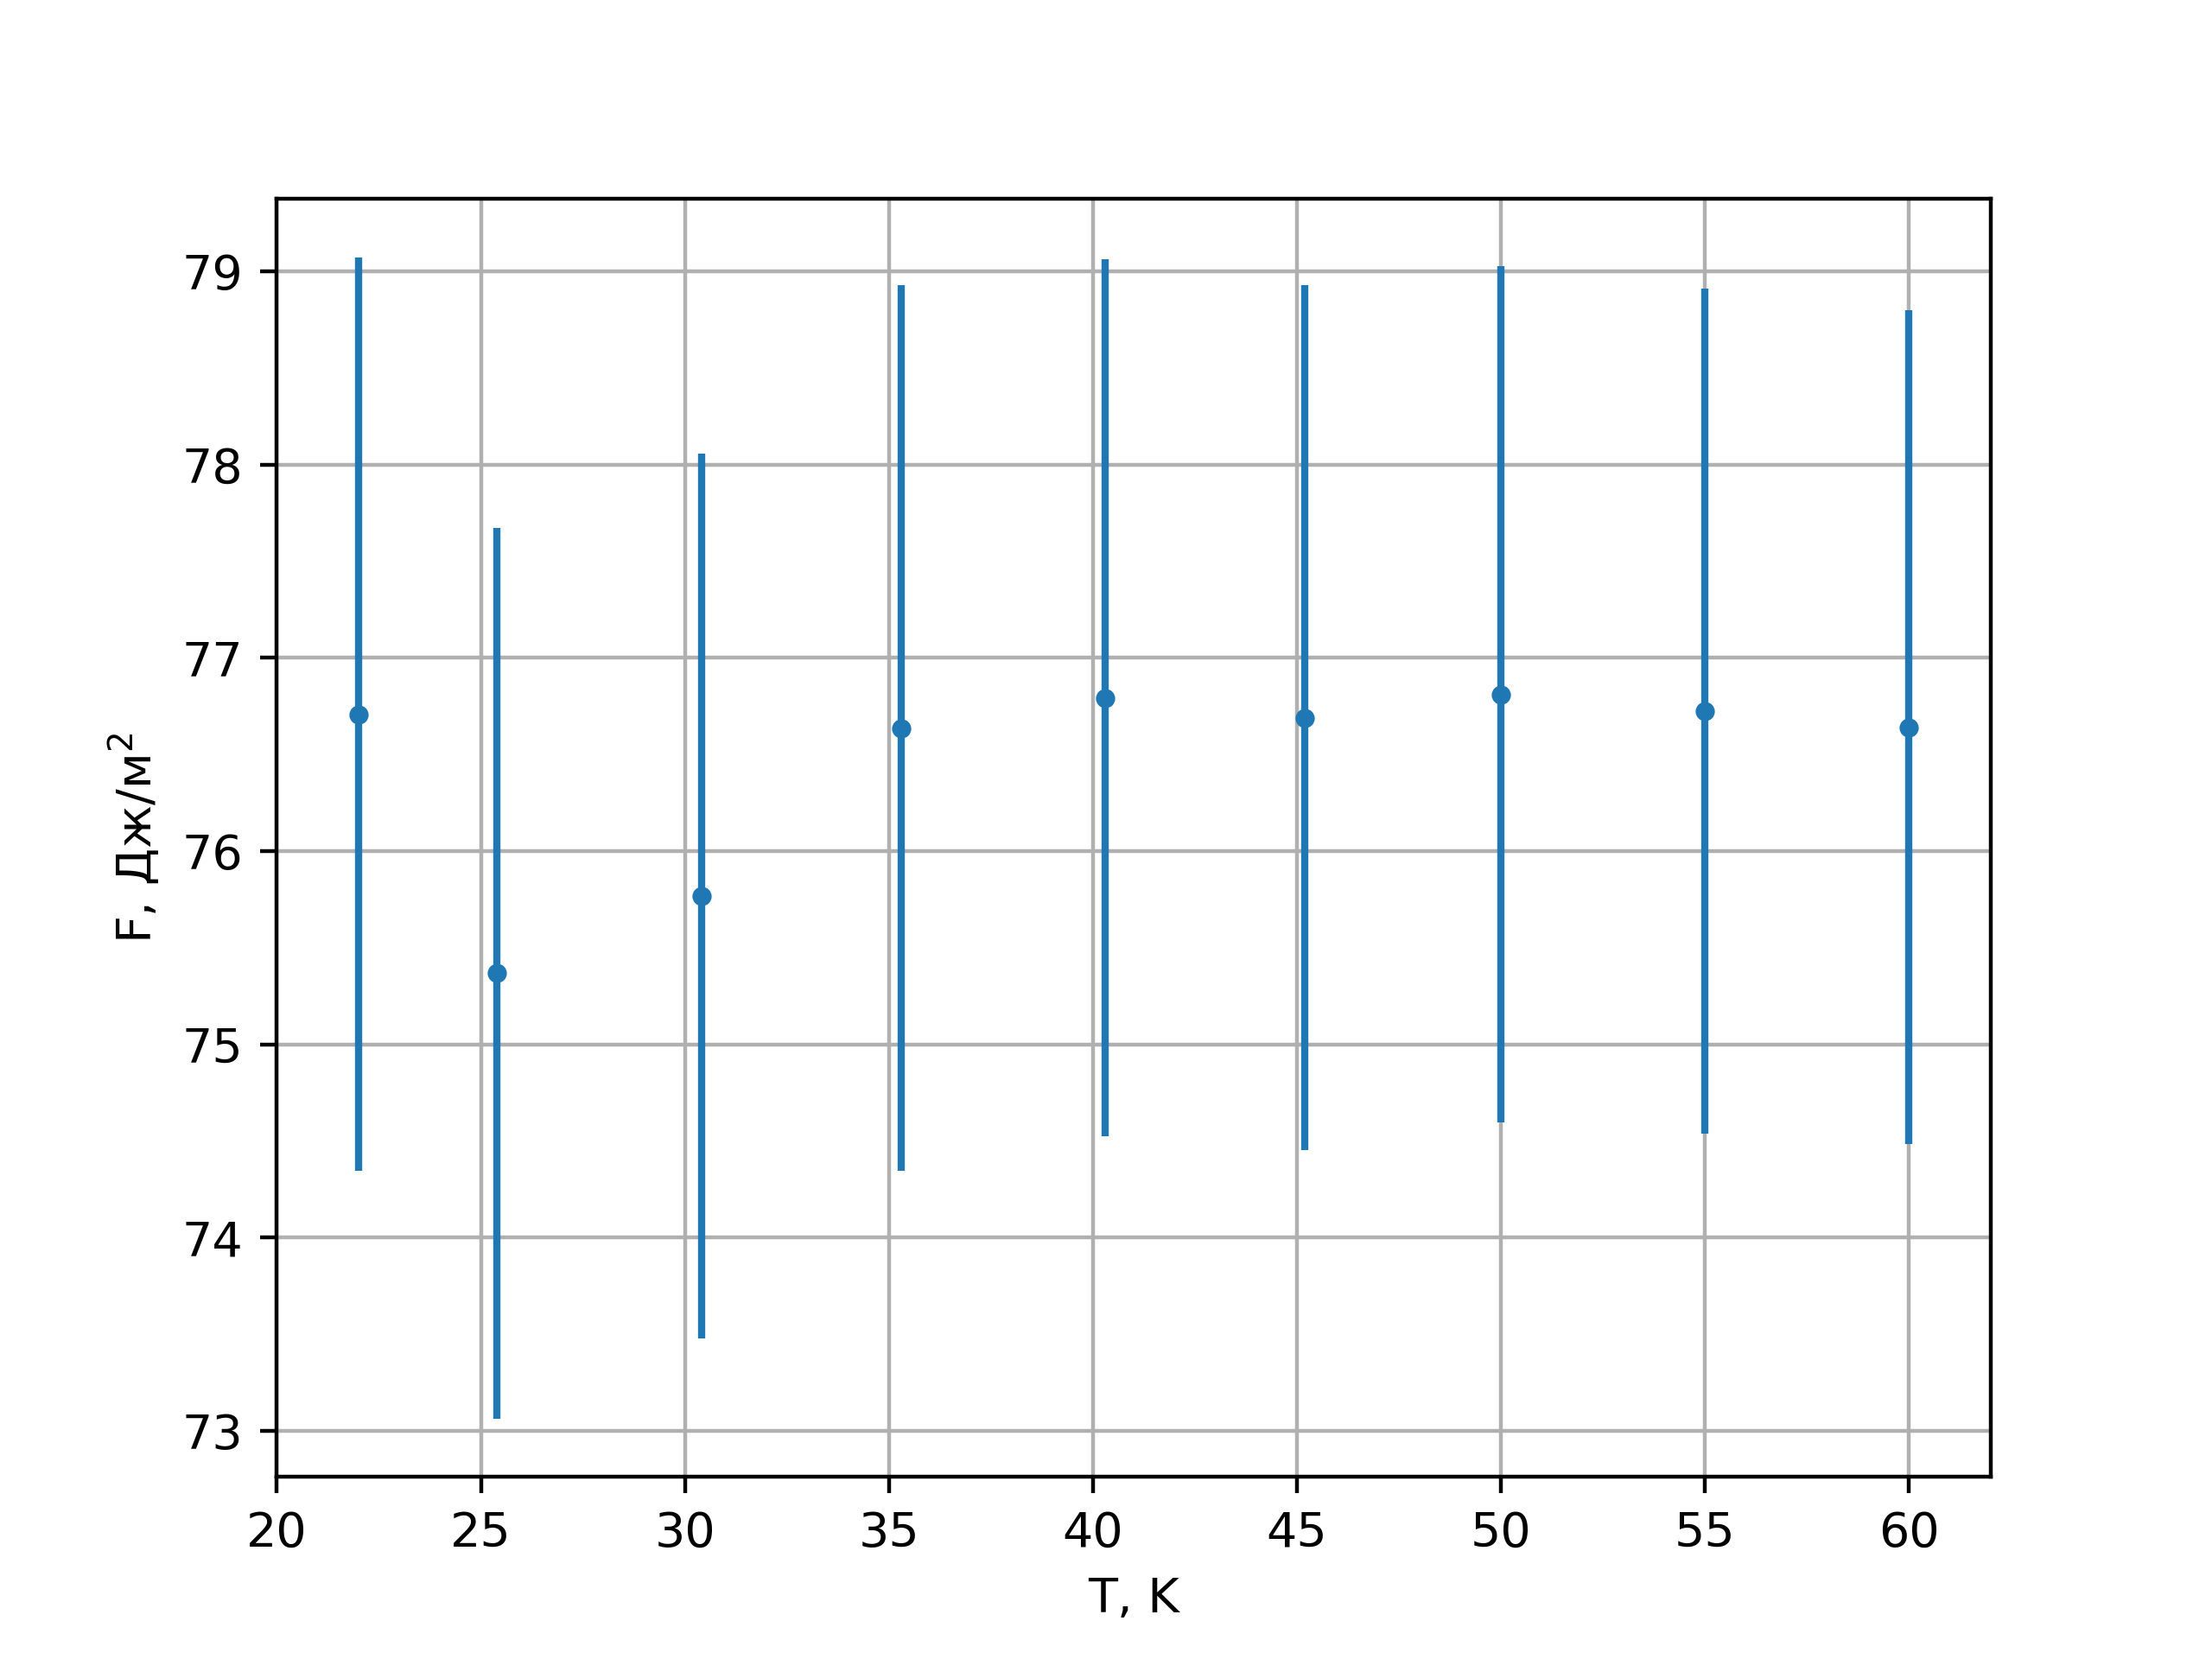
\includegraphics[width=0.8\linewidth]{img/plot3.png}
\end{figure}

\newpage
~
\newpage